% A sample UCalgary-branded poster using tikzposter

\documentclass{tikzposter} % Options for format can be included here

\usepackage{ucalgary-poster}

% Make the size 60 by 42"
\geometry{paperwidth=60in,paperheight=42in}
\tpsetpostersize

% Make the body font a bit larger (33pt)
\def\large{\fontsize{33}{40}\selectfont}

% Why not have links?
\usepackage[hidelinks]{hyperref}

% Title, Author, Institute

\title{Evaluation of a Student-Oriented Logic Course}
\author{Aaron Thomas-Bolduc, Richard Zach}
\institute{Department of Philosophy}

\begin{document}

 % Title block with title, author, logo, etc.
\maketitle

% Layout: we use 4 columns, each .25 of textwidth
\begin{columns}

% First column
\column{0.25}

\block{Challenge}{Courses in formal logic are taught in most
  English-speaking philosophy departments. Yet very little effort
  seems to have been made to deliver these courses in a way that
  improves learning outcomes.  A typical introductory course in formal
  logic still involves a standard lecture format, with tutorials,
  problem sets and closed book exams. Textbooks tend to be pricey
  (\$100 and up).  Logic courses often have a highly skewed gender
  split, and instructors face the issue of teaching to a wide range of
  student backgrounds and expectations. Grade distributions are lower 
  than average for philosophy courses, and the DFW (D-F-withdraw) 
  rate is high.}

\block{Context}{Most scholarship on the instruction of elementary
  logic (Croy 2010; Geach 1979; Hedges 1999; Schiller 1913) has
  assumed the traditional lecture model. One notable exception is
  Butchart et al.\ (2009) who investigated the implementation of peer
  instruction. They found that peer instruction provided statistically
  significant increases in student satisfaction and learning outcomes
  as compared to the traditional lecture model of instruction. The
  meta-analysis in Macpherson (2016) reports that students who score
  highly for maths anxiety have worse learning outcomes than more
  confident students, and suggests that cooperative learning decreases
  maths anxiety and its effects.  Cooperative learning is integral to
  both peer instruction and classroom flipping.}

\block{New Logic Course}{In Winter 2017, the first author piloted a
  course in formal logic in which we aimed to (a) improve student
  engagement and mastery of the content, and (b) reduce maths anxiety
  and its negative effects on student outcomes, by adopting student
  oriented teaching including peer instruction and classroom flipping
  techniques. The course implemented a partially flipped approach, and
  incorporated group-work and peer learning elements, while retaining
  some of the traditional lecture format. By doing this, a wide
  variety of student learning preferences could be provided for.}

\block{Open Textbook}{We revised and remixed a free and open source
  textbook, \emph{forall x} (Magnus et al. 2017) which was used as the
  primary text. We evaluated student satisfaction using a survey
  instrument based on the Textbook Assessment and Usage Scale (Gurung
  and Martin 2011), and compared it to student satisfaction with the
  traditional textbooks in use in other sections of the course
  (Chellas 1997, Goldfarb 2013). The survey also asked about use
  patterns, e.g., how often students consulted the textbook, for what
  purpose the consulted the text, and how they interacted with
  it. (For \emph{forall x}, $n = 25$; Chellas, $n=31$; Goldfarb,
  $n=45$.)  The survey was approved by the Conjoint Faculties Research
  Ethics Board.}

% Second column
\column{0.25}

\block{Textbook Use}{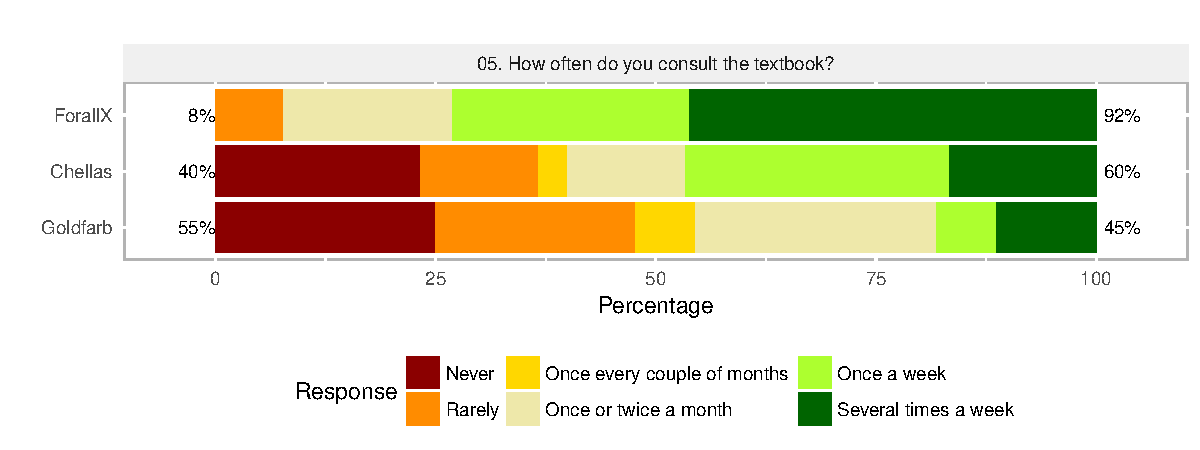
\includegraphics[width=.22\textwidth]{Rplot05.pdf}}

\block{Student Satisfaction}{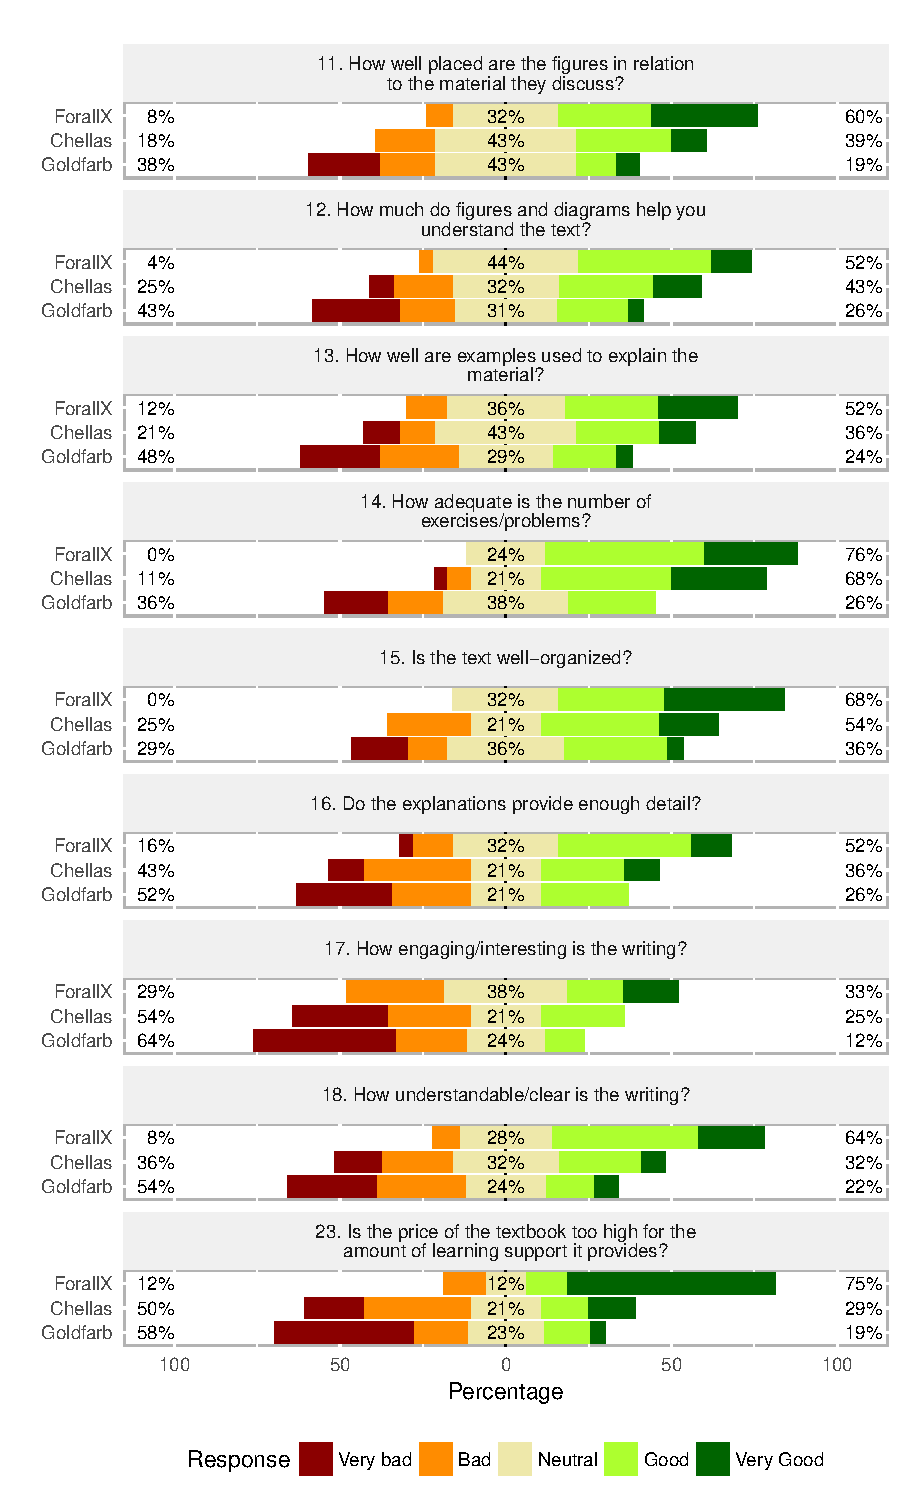
\includegraphics[width=.22\textwidth]{Rplot04.pdf}}

% Third column
\column{0.25}
  
\block{Partially Flipped Classroom}{The flipped portion of class
  involved providing short (5--6~min) screencasts a few days before
  scheduled groupwork. The groupwork then covered material from the
  screencast as well as from the previous 2--3 lectures. Students were
  also expected to read the relevant portions of the textbook. The
  screencasts themselves were online videos with the instructor's
  scripted voice recorded over slides, covering central concepts and
  themes. The students thus learned a good deal of material via
  screencasts, peer learning during groupwork, and the textbook.}
  
\block{Groupwork}{The students were put into groups of 5 or 6 based on
  their tutorial sessions, and upper level students were distributed
  as evenly as possible. Dividing the students by tutorial session
  allowed the assignments to be completed over the course of one class
  session plus one tutorial. This way, students always had access to
  the instructor or TA, and needn't get together outside of class
  times. Groupwork assignments generally had fewer, but difficult or
  open-ended questions. This was meant to encourage collaboration and
  discussion, as well as to expose the students to more advanced
  material when they were able to ask questions.}

\block{Other Course Components}{Generally 1--2 classes per week were
  traditional lectures, though these were often broken up by other
  activities, some of which included brief group discussions. There
  were also 3 in-class tests, and 6 homework assignments. Homework was
  completed over one week, and generally consisted of many shorter
  questions. Finally, there was a participation component based
  primarily on groupwork, which included peer evaluation.}

\block{D--F--Withdraw Rates}{The DFW rates for the 10 sections of
  Logic I in 2014/15 and 2015/16 ranged from 8\% to 36.7\%, with mean
  23.4\% and median 23.7\%. The DFW rate for this course was
  7.9\%. This is in line with the two lowest rates (8\%, 8.3\%), but
  those were outliers, the next lowest being 18\%. This suggests that
  our approach may help retain students.}

\block{Limitations}{Validity of survey results and DFW rates may be
  limited by a number of factors. Differences in textbooks and
  instructor between sections were not controlled for, nor were
  methods of evaluation. This was possibility confounded by the fact
  that this was the instructor's first time teaching. Surveys were
  prone to selection bias. Timing of the course (Winter term,
  afternoons) may have provided an unrepresentative sample of Logic I
  students.}

% Fourth column
\column{0.25}

\block{Student Evaluation}{With CFREB approval, we added questions to
  the standard faculty teaching evaluation form to gauge student
  satisfaction with the revised format of the course ($n = 55$).

  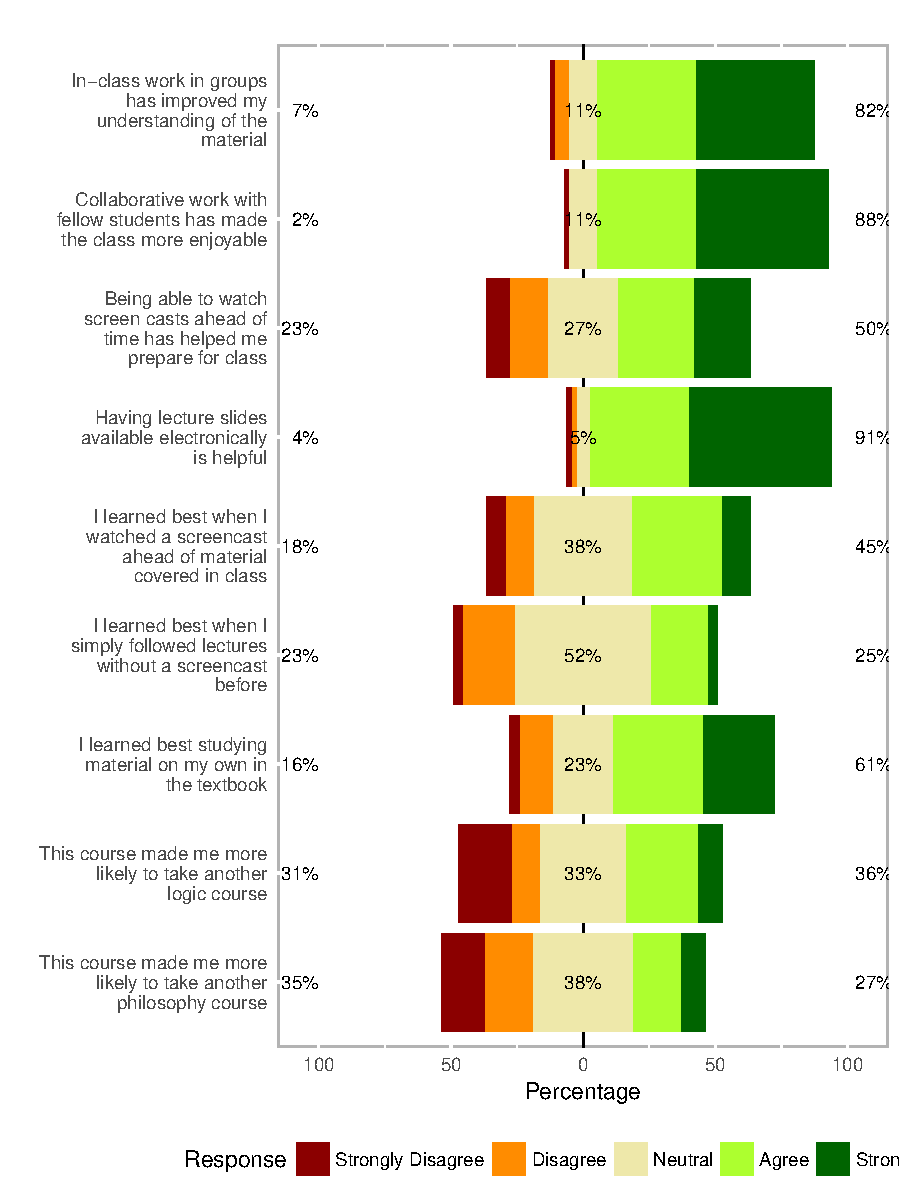
\includegraphics[width=.22\textwidth]{Rplot06.pdf}}

\block{Discussion}{Despite the mentioned limitations, the very
  positive responses to both the book and the course structure suggest
  that this method of teaching logic, and the chosen open textbook
  \textit{forall x}, help improve learning outcomes and student
  retention. In the instructor's opinion, groupwork in particular was
  genuinely helpful for students.}

\block{References}{\raggedright\fontsize{20}{23}\selectfont
  \begin{list}{}{\setlength{\itemindent}{-2em}\setlength{\leftmargin}{2em}}
  \item S. Butchart, T. Handfield, G. Restall (2009). Teaching
    Philosophy, Logic and Critical Thinking using Peer
    Instruction. \emph{Teaching Philosophy}~32:1-40.
  \item B. Chellas (1997). \emph{Elementary Formal Logic}, Penny Lane.
  \item M. J. Croy (2010). Teaching the Practical Relevance of
    Propositional Logic. \emph{Teaching Philosophy}~33:253-270.
  \item P. T. Geach (1979). On Teaching Logic. \emph{Philosophy}~54:5-17.
  \item W. Goldfarb (2013). \emph{Deductive Logic}. Hackett.
  \item R. A. R. Gurung, R. C. Martin (2011). Predicting Textbook
    Reading. \emph{Teaching of Psychology}~38:22--28.
  \item S. Hedges (1999). Do Students Learn in My Logic Class?
    \emph{Teaching Philosophy}~22:141-159.
  \item B. Macpherson (2016). Overcoming Instructor-Originated Math
    Anxiety in Philosophy Students. \emph{Metaphilosophy}~47:122-146.
  \item P. D. Magnus et al. (2017). \emph{forall x: Calgary
    Remix}. \href{http://forallx.openlogicproject.org/}{forallx.openlogicproject.org}
  \item J. McGivney-Burellee, F. Xue (2013). Flipping
    Calculus. \emph{PRIMUS}~23: 477--486.
  \item F. C. S. Schiller (1913). The Social Value of Logic
    Teaching. \emph{Hibbert Journal}~12:192.
\end{list}
}

\end{columns}

% Footer
\footer[width=\paperwidth,height=7cm]{
  % Needs a bit more space for the logos
  \hspace{1.5cm}
  % Since we have two sponsors, UCalgary brand guidelines say we
  % should use wordmarks not lockups
  \begin{minipage}{.5\textwidth}
    
\includegraphics[height=4cm]{ti-wordmark.pdf}
    \hspace{.1\textwidth}
    
\includegraphics[height=4cm]{philosophy-wordmark.pdf}
  \end{minipage}
  \hfill
  \begin{minipage}{.2\textwidth}
    Research supported by the Taylor Institute for Teaching and
    Learning through a Scholarship of Teaching and Learning Grant, and
    by the Department of Philosophy.
  \end{minipage}
  \hfill
  \begin{minipage}{.25\textwidth}
    \raggedleft \textbf{Contact Information}\\
    Aaron Thomas-Bolduc\\
    athomasb\@ucalgary.ca
  \end{minipage}\hspace{1.5cm}
}

\end{document}


